\chapter{Setting Up the Input File for CFAST}

\section{Overview}

CFAST is a computer program that uses an input file and generates one or more output files. The first step in performing a calculation is to generate a text input file that provides the program with all of the necessary information to describe the scenario under consideration.  The most important inputs determine the geometry of the compartments in the scenario and the connections between these compartments. Next, the fire, detection, and suppression characteristics of the scenario are defined. Finally, there are a number of parameters that customize the output from the model.  Each line of the file contains a keyword label that identifies the input, followed by a number of numerical or text inputs corresponding to the particular input keyword. A simple input file is shown below. This example is used in the discussion of the output in Chapter 5.

\begin{lstlisting}
VERSN,6,Cable tray fire -- base case
TIMES,1800,120,0,30
EAMB,293.15,101300,0
TAMB,293.15,101300,0,50
LIMO2,10
WIND,0,10,0.16
COMPA,Compartment 1,9.1,5,4.6,0,0,0,GLASSFB3,CONCRETE,CONCRETE
HVENT,1,2,1,1,2.4,0,1,0,0,1,1
OBJECT,bunsen,1,4.55,2.5,0,1,1,0,0,0,1
OBJECT,Wood_Wall,1,4.55,2.5,0,1,1,0,0,0,1
TARGET,1,2.2,1.88,2.34,0,0,1,CONCRETE,IMPLICIT,PDE
\end{lstlisting}

All of the inputs to the model are discussed in this chapter.  Following the discussion that details each input, their engineering units and default values, notes are included that provided additional guidance or frequently addressed problems that may be encountered by the user. These notes take the form of a bulleted list such as:

\begin{itemize}
\item The inputs may be integers (e.g., a simulation time of 1800 s), real numbers (a mass loss rate of 0.0082 kg/s), or text (a floor material of CONCRETE), as appropriate. The input file is a comma-separated ASCII text file and may be edited with a spreadsheet program or any text editor. It is possible to use a word processor but it is important to save the file in ASCII text format and not in a word processing format. Note that some word processors will save punctuation and other characters incorrectly for the simple ASCII text file used by CFAST. It is recommended that the input files be created with the input editor, CEdit, provided as part of the CFAST distribution.  In addition to checking the input data for errors, it includes typical ranges for input values to assist in appropriate use of the model.

\item Numeric format for inputs to CFAST and the input editor CEdit assume a period is used to separate the integer and fractional parts of the number. No separator is used to group digits in the integer part of numbers.

\item Each line of input consists of a label followed by one or more alphanumeric parameters associated with that input label, separated by commas.  The label must always begin in the first space of the line and be in capital letters.  Following the label, the values may start in any column, and all values must be separated by a comma.  Values may contain decimal points if needed or desired.  They are not required.  

\item Inputs are in standard SI units.  The maximum line length is 1024 characters, so all data for each keyword must fit in this number of characters.
\end{itemize}

The installation program creates a shortcut to the input editor on the Windows start menu labeled �CFAST� that points to the input editor.  Once started, the user is presented with a series of tabbed-pages for the various inputs in a CFAST input data file.

\begin{figure}[h!]
\begin{center}

\includegraphics[width=6.5in]{FIGURES/Input_File/Tabs}
\end{center}
\end{figure}

These tabbed-pages organize the inputs for CFAST simulations into several categories as follows.
\begin{itemize}
\item \textbf{Simulation Environment} includes simulation time, specification of model outputs, and ambient conditions. Also included on the page are a constantly updated list of errors, warnings, and messages about the input file specification or model simulation.
\item \textbf{Compartment Geometry} defines the size, construction characteristics, and position of the compartments in a simulation.
\item \textbf{Wall Vents, Ceiling/Floor Vents, and Mechanical Flow Vents} allows the user to connect compartments with doors and windows, ceiling and floor vents, or forced air ventilation systems.
\item \textbf{Fires} include user specification of the initial fire source and any additional burning objects in one or more of the compartments of the simulation.
\item \textbf{Detection / Suppression}defines any heat alarms and sprinklers in the compartments of the simulation.
\item \textbf{Targets} provide the ability calculate the temperature and net heat flux to objects placed and oriented arbitrarily in the structure.
\item \textbf{Surface Connections} allows for more detailed description of the connections between compartments in the simulation to better simulate the transfer of heat from compartment to compartment in the simulation.
\end{itemize}

Each of these tabbed-pages is described in more detail below. In addition, a series of menus allow the user to open and save files; run the simulation, or access help and program information.

\section{Simulation Environment}

The Simulation Environment page defines the initial conditions and simulation time for the CFAST input file. 

\begin{figure}[h!]
\begin{center}
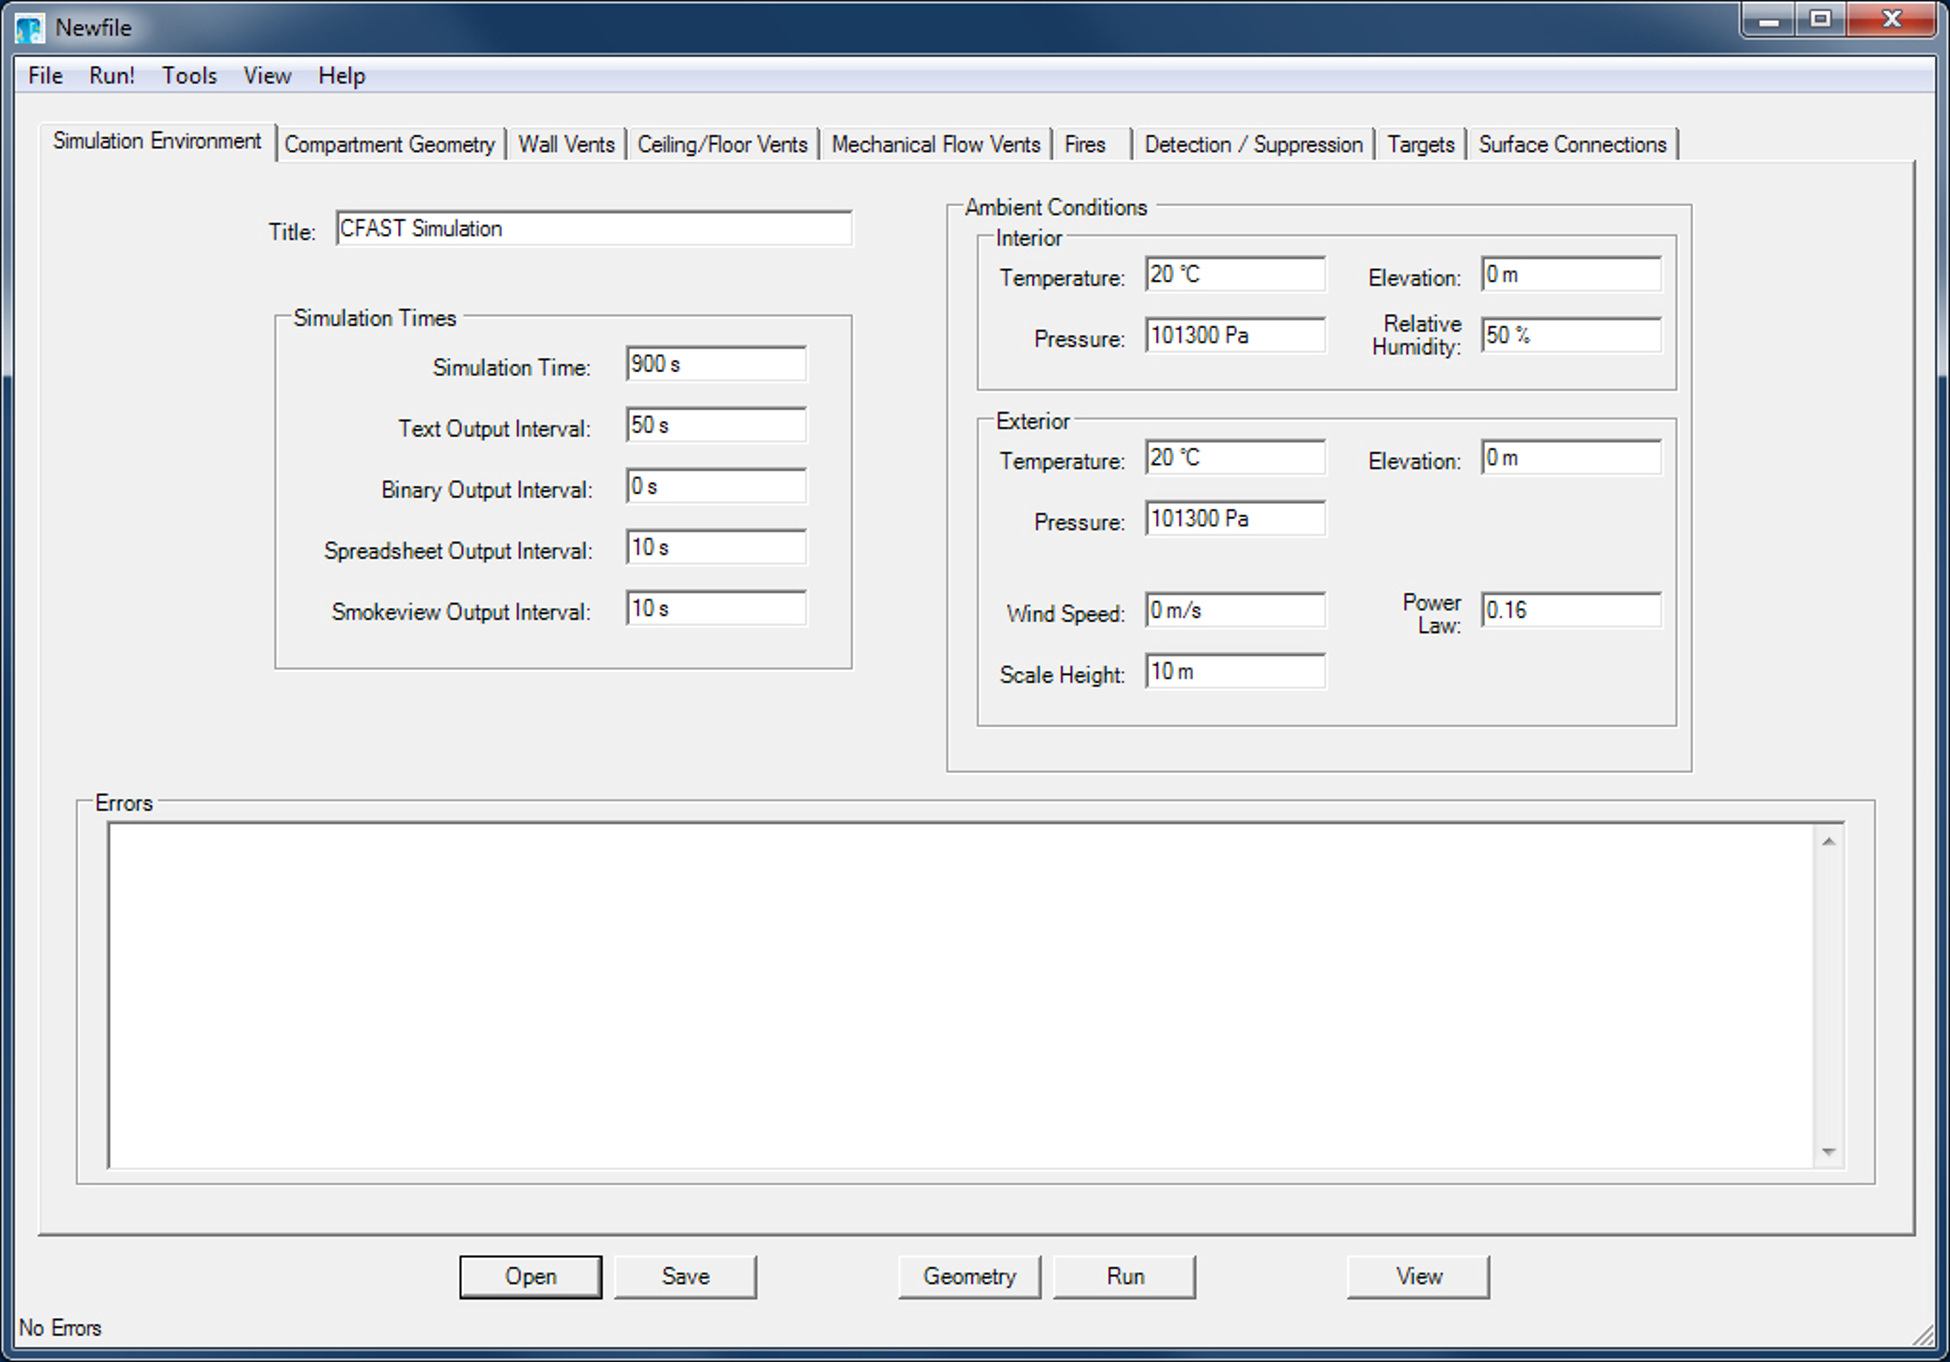
\includegraphics[width=6.5in]{FIGURES/Input_File/Environment_Tab}
\end{center}
\end{figure}

\subsection{Naming the Calculation, the Title Input}

The first thing to do when setting up an input file is to give the simulation a title.  The first line in the CFAST input data file must be the CFAST version identification along with an optional short title for the simulation.  This is a required input.  The title command is the line that CFAST keys on to determine whether it has a correct data file.

\begin{lstlisting}
VERSN,6,CFAST Simulation
\end{lstlisting}

\clearpage

\begin{figure}[h!]
\begin{center}

\includegraphics[width=3.458in]{FIGURES/Input_File/Title}
\end{center}
\end{figure}

\textbf{Title:} The title is optional and may consist of letters, numbers, and/or symbols and may be up to 50 characters. It permits the user to label each run.

\subsection{Setting Time Limits and Output Options}

A TIMES line specifies the length of time over which the simulation takes place and how often output will be generated. This is a required input. There are one to four entries in this line.

\begin{lstlisting}
TIMES,900,50,10,10
\end{lstlisting}

\begin{figure}[h!]
\begin{center}
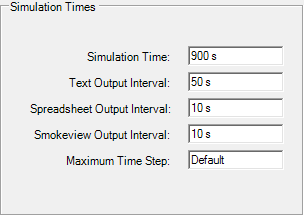
\includegraphics[width=3.167in]{FIGURES/Input_File/Simulation_Times}
\end{center}
\end{figure}

\begin{itemize}
\item \textbf{Simulation Time} (default units: s, default value, 900 s): The length of time over which the simulation takes place.  This is a required input which should be entered even if all other fields are not included. The maximum value for this input is 86400 s (1 day).

\item \textbf{Text Output Interval} (default units: s, default value, 50 s): The print interval is the time interval between each printing of the output values.  If omitted or less than or equal to zero, no output values will occur.

\item \textbf{Spreadsheet Output Interval} (default units: s, default value, 10 s): CFAST can output a subset of the results of the model simulation in a comma-delimited alphanumeric format which can be read by most spreadsheet software. This is designed to be imported into a spreadsheet for further analysis or graphing of the results of the simulation.  This input defines the time interval between outputs of the model results in a spreadsheet-compatible format. A value greater than zero must be used if the spreadsheet file is to be used.

\item \textbf{Smokeview Output Interval} (default units: s, default value: 10 s): CFAST can output a subset of the results in a format compatible with the visualization program smokeview. This input defines the time interval between outputs of the model results in a smokeview-compatible format.  A value greater than zero must be used if the spreadsheet output is desired.
\end{itemize}

In addition to the input data file created specifically for a CFAST simulation, there are a number files that CFAST uses to define default values and other input information, and to output the results of the simulation for later analysis.  They include 1) a thermal properties file, 2) files of predefined fire objects, and 4) a spreadsheet-compatible output file.

The thermal properties file contains material properties for compartment surfaces, target objects that may be placed in compartments in the simulation to monitor surface temperature and heat flux to the objects, and fire objects, in addition to the main fire in the simulation that may ignite based on their surface temperature or incident flux onto the surface of the object. The predefined fire objects files contain definitions for a number of reference fires from the literature or developed by the user that may be included in a simulation. The thermal properties and fire objects files may be modified by the user.  Details of the files are included in the appendices.  There are default files included in the CFAST distribution.

\subsection{Ambient Conditions}

Ambient conditions define the environment at which the scenario begins. This allows the user to specify the temperature, pressure, and station elevation of the ambient atmosphere, as well as the absolute wind pressure to which the structure is subjected.  Pressure interior to a structure is calculated simply as a lapse rate (related to the height above sea level) based on the NOAA/NASA tables \cite{GPO:Atmosphere}.  This modification is applied to the vents which connect to the exterior ambient.  The calculated pressure change is modified by the wind coefficient for each vent.  This coefficient, which can vary from -1.0 to +1.0, nominally from -0.8 to +0.8, determines whether the vent is facing away from or into the wind.  The pressure change is multiplied by the vent wind coefficient and added to the external ambient for each vent which is connected to the outside. There is an ambient for the interior and for the exterior of the structure.  Three keywords define the ambient conditions: TAMB for the interior of the structure, EAMB for the exterior of the structure is EAMB, and WIND for the wind information.

\begin{lstlisting}
EAMB,293.15,101300,0
TAMB,293.15,101300,0,50
WIND,0,10,0.16
\end{lstlisting}

\begin{figure}[h!]
\begin{center}
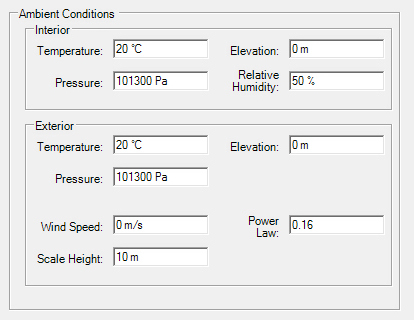
\includegraphics[width=4.313in]{FIGURES/Input_File/Ambient_Conditions}
\end{center}
\end{figure}

\textbf{Ambient Temperature} (default units: �C, default value: 20 �C): Initial ambient temperature inside (for TAMB) or outside (For EAMB) the structure at the station elevation.

\textbf{Ambient Pressure} (default units: Pa, default value: 101300 Pa): Initial values for ambient atmospheric pressure inside (for TAMB) and outside (for EAMB) the structure at the station elevation. Default value is standard atmospheric pressure at sea level (0 m elevation) of 101.3 kPa. Input units are in Pa. These values define standard conditions as defined in Standard Atmosphere as noted in the Handbook of Chemistry and Physics  . There is a set of numerical approximations in the CFAST code which duplicate the pressure/temperature/altitude relationships in the handbook.

\textbf{Elevation} (defaults units: m, default value: 0 m): The height where the ambient pressure and temperature were specified.  This is the reference datum for calculating the density of the atmosphere as well as the temperature and pressure inside and outside of the structure as a function of height.  

\textbf{Relative Humidity} (default units \% RH, default value: 50 \%): The initial relative humidity in the system, only specified for the interior with the TAMB command.  This is converted to kilograms of water per cubic meter.

The wind speed, scale height, and power law are used to calculate the wind coefficient for each vent connected to the outside.  The wind velocity is specified at some reference height.  The power law then provides a lapse rate for the wind speed.  An assumption is that the wind speed is zero at the surface.  The formula used to calculate the wind speed at the height of any vent is show below.  The wind is applied to each external opening as a change in pressure outside of the vent.

\textbf{Wind Speed} (default units: m/s, default value 0 m/s): Wind speed at the reference elevation.

\textbf{Scale Height} (default units: m, default value: 0 m)): Reference height at which the reference wind speed is measured.

\textbf{Power Law Coefficient} (default units: dimensionless, default value 0.16): The power law used to calculate the wind speed as a function of height. Default value is 0.16. Using the notation that $V_W$, is the wind speed at the reference height $H_W$, and $P_W$ is the power law, the exterior pressure is modified by  $\delta P = {C_W}{V^2}$ and $V = {V_W}{\left( {\frac{{{H_i}}}{{{H_W}}}} \right)^{{P_W}}}$ where $H_i$ is the position of the vent \cite{CFAST_Tech_Guide_6}.

\begin{itemize}
\item In order to see the effect of wind, the corresponding parameter for the ventilation keyword must be specified. The default for the wind vector is 0, which turns off wind effects. Please see the HVENT command, below.

\item The choice for station elevation, temperature and pressure must be consistent.  Outside of that limitation, the choice is arbitrary.  It is often convenient to choose the base of a structure to be at zero height and then reference the height of the structure with respect to that height.  The temperature and pressure must then be measured at that position.  Another possible choice would be the pressure and temperature at sea level, with the structure elevations then given with respect to mean sea level.  This is also acceptable, but somewhat more tedious in specifying the construction of a structure.  Either of these choices works though, so long as they are consistent. Usually, the station elevation is set to zero and the pressure to ambient. The effect of changing these values is small for small changes. There will be an effect for places at altitude such as Denver, Colorado, but even there the effect is not pronounced. Note that the equations implemented in the model are not designed to handle negative elevations and altitudes. It is suggested that the defaults be used.

\item These three parameters are optional. If they are not included in the input file, default values are used.
\end{itemize}

\section{Compartment Geometry}

The Compartment Geometry page defines the size, position, materials of construction, and flow characteristics for the compartments in the simulation. Initially, only the simulation environment page and the �Add� button on the compartment geometry page is enabled; all other pages are not available to the user for detailed inputs until a compartment has been added to the simulation.  

\begin{figure}[h!]
\begin{center}
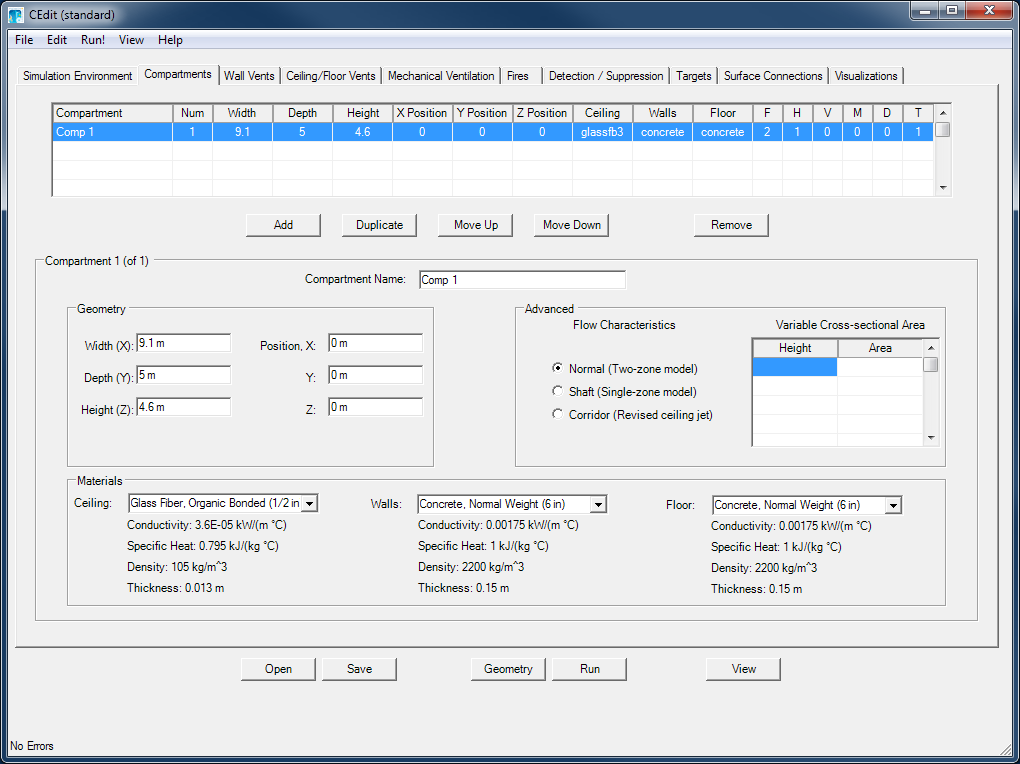
\includegraphics[width=6.5in]{FIGURES/Input_File/Compartment_Geometry_Tab}
\end{center}
\end{figure}

Most of the tabbed pages in the program are of similar design, with a summary of the defined items in table form at the top of the page, a series of buttons to add, remove, or modify the item highlighted in the summary table, and a number of individual inputs below which details all of the inputs for the item selected in the summary table. The buttons included on the compartment geometry page are as follows:
